\chapter{Controlador de corriente} \chapterlabel{Informe/4-ControladorCorriente} \label{cap:ControladorCorriente}

En este capítulo se diseña y modela el circuito encargado de controlar la corriente que circula por el electroimán. Como se vio en el capítulo anterior, el sistema trabaja con corrientes elevadas por lo que se implementan estrategias de conmutación para reducir las pérdidas de energía. Para ello se utiliza una topología de puente H con cuatro MOSFET y un \textsl{driver} que los controla. Además, se detallan los criterios tenidos en cuenta al momento de  elegir  y dimensionar todos los componentes que intervienen para lograr el correcto funcionamiento del controlador de corriente. Por último, se obtiene su función transferencia  para ser utilizada en el diseño del compensador.

\section{Descripción general}

Para mantener en suspensión a la pieza móvil es necesario regular la fuerza electromagnética generada por el electroimán. Esto se logra modificando la intensidad de la corriente que circula por su bobinado. Para ello, es necesario diseñar una fuente de alimentación que sea capaz de proveer la corriente requerida.

Para diseñar la fuente de alimentación se debe conocer el comportamiento eléctrico de la planta. Como se analizó en el capítulo \ref{cap:CaracterizacionElectroiman}, el electroimán puede ser modelado como una inductancia variable con una resistencia serie. Es decir, es un circuito RL serie cuya corriente ($I_L$) depende de la tensión aplicada ($V_L$). La expresión \ref{eq_corriente} muestra la relación entre estos parámetros.

\begin{equation} \label{eq_corriente}
\frac{I_L}{V_L}(s)=\frac{1}{sL(Y_g)\ +\ R_L}
\end{equation}

Al aplicar la transformada inversa de Laplace a la expresión  \ref{eq_corriente}, se puede obtener la respuesta temporal de la corriente ante un escalón de tensión de amplitud ``$v_L$'' en la entrada:

\begin{equation} \label{eq_corriente_temporal}
	i_L(t)=\frac{v_L}{R_L}*(1-\frac{1}{L(Y_g)}*e^{-\frac{R_L}{L(Y_g)}*t})
\end{equation}

\colorbox{red}{revisar lo de arriba}En la expresión \ref{eq_corriente_temporal} se puede observar que la respuesta al escalón está compuesta por dos partes: un término con una exponencial negativa correspondiente al transitorio, y un término constante correspondiente al valor en régimen permanente $\frac{v_L}{R_L}$. El primero provoca que la corriente en el inductor crezca de manera amortiguada, hasta alcanzar el valor de régimen permanente luego de cierto tiempo. Este comportamiento se puede observar en la simulación realizada en la figura \ref{fig:img_respuesta_escalon}. En la parte superior de la figura se observa la tensión de entrada, y en la parte inferior la corriente del electroimán. Este análisis resulta de utilidad para conocer el comportamiento del electroimán y diseñar un controlador de corriente adecuado.


\begin{figure}[H]
	\centering
	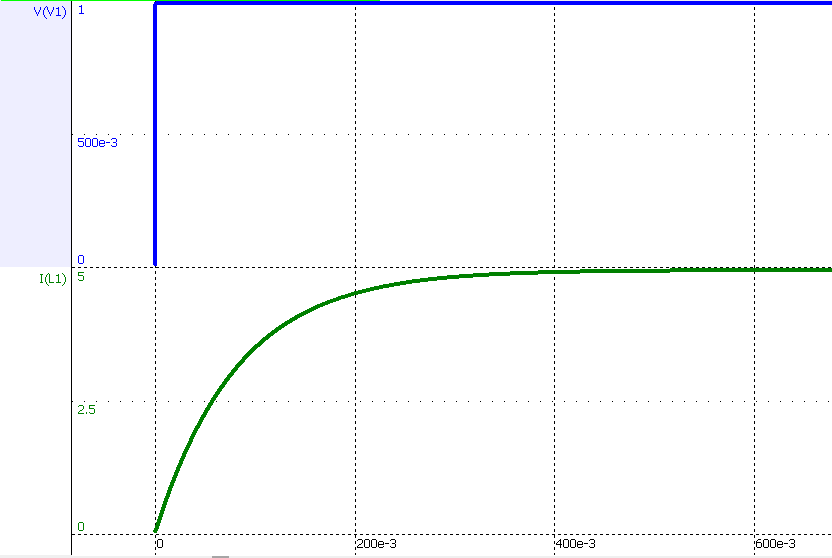
\includegraphics[scale=0.5]{corriente_escalon.png}
	\caption{Respuesta ante una entrada en escalón.}
	\label{fig:img_respuesta_escalon}
\end{figure}


\section{Diseño de topología}


Se desea diseñar un sistema de control que modifique la alimentación del electroimán con el objetivo de que circule una corriente específica por su bobinado.  Para ello, se implementa un sistema realimentado que compara la corriente que circula por el electroimán con una de referencia, que es la que se desea que circule por el electroimán. En la figura \ref{fig:img_diagrama_bloques_basico} se muestra un diagrama en bloques inicial del sistema.


\begin{figure}[H]
	\centering
	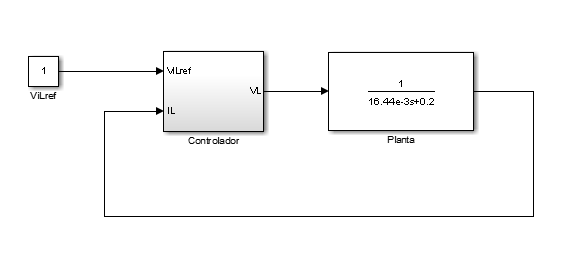
\includegraphics[scale=1]{Diagrama-en-bloques-basico.png}
	\caption{Diagrama en bloques básico del controlador de corriente.}
	\label{fig:img_diagrama_bloques_basico}
\end{figure}

\colorbox{red}{Acá estaría bueno proponer} que vamos a analizar dos manera de controlar la corriente. o alguna intro similar

\subsection{Control de corriente mediante transistor en modo lineal}

Como se vio en la introducción del capítulo, el valor en régimen permanente de la corriente depende proporcionalmente de la tensión aplicada al electroimán. Por lo tanto, 

Para mantener una corriente constante controlada se podría utilizar un transistor en modo lineal, es decir, como una fuente de corriente constante. Una posible implementación circuital se muestra en la figura \ref{fig:img_controlador-lineal}.

\begin{figure}[H]
	\centering
	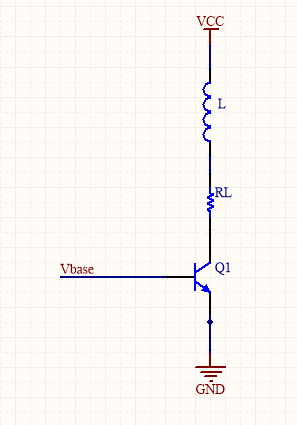
\includegraphics[scale=0.7]{controlador_lineal.png}
	\caption{Control de corriente mediante transistor en modo lineal.}
	\label{fig:img_controlador-lineal}
\end{figure}

En este modo de funcionamiento la tensión colector-emisor ($V_{CE}$) se controla de manera que la diferencia entre esta y la tensión de alimentación, circulando por la resistencia interna del electroimán, generen la corriente deseada. Es decir, en régimen permanente se obtiene:
 
 \begin{equation} \label{eq_corriente_temporal}
 	I_L=\frac{V_{CC}-V_{CE}}{R_L}
 \end{equation}
 
La desventaja de esto es que al circular una corriente constante, la caída de tensión sobre el inductor es prácticamente nula (solo lo correspondiente a la resistencia interna). Por lo tanto, la mayor parte de la potencia disipada cae sobre el transistor. Esta puede calcularse como: 

\begin{equation}
	P_{transistor} = I_L*V_{CE}
\end{equation}

Teniendo en cuenta que la tensión colector-emisor es la resta de la tensión de alimentación y la caida en la resistencia del electroimán:

\begin{equation}
	V_{CE}=V_{CC}-I_L*R_L
\end{equation}

Finalmente:

\begin{equation}
	P_{transistor}=V_{CC}*I_L-I_L^2*R_L
\end{equation}

Esta función llega a un máximo cuando $I_L=\frac{V_{CC}}{2*R_L}$


\begin{equation}\label{eq_pot_transistor_lineal_final}
	P_{transistor_{max}}=\frac{V_{CC}^2}{4*R_L}
\end{equation}

Teniendo en cuenta que la corriente maxima que se requiere es de aproximadamente 30 A se puede obtener que la minima tension de VCC requerida es:

\begin{equation}
	V_{CC}=I_L*R_L+V_{CE}=30 A * 0,2  = 5 V, VCE=0
\end{equation}

En el mercado las fuentes de tension capaces de entregar 30 A mas comunes en el mercado comienzan con valores minimos de 12 V. Si se reemplaza este valor en la ecuacion  \ref{eq_pot_transistor_lineal_final} se obtiene un valor minimo de 180 Watt, esto elevaria demasiado la temperatura del transistor, haciendo que sea necesario el agregado de un gran disipador de calor y pone en riesgo la vida útil de los componentes.
  
En la ecuación \ref{eq_pot_transistor_lineal_fina} se puede ver que para valores de tension normalmente utilizados $(5\:V,10\:V,15\:V)$ la potencia disipada por el transistor varía entre $30\:W$ hasta $280\:W$. Esto eleva demasiado la temperatura del transistor, haciendo que sea necesario el agregado de un gran disipador de calor y pone en riesgo la vida útil de los componentes.

Aunque aún no se define con qué tensión se alimentará el sistema, se puede probar con valores utilizados comunmente para obtener una aproximación de la potencia disipada por el transistor. Por ejemplo, para valores de tensión de alimentación $(5\:V,10\:V,15\:V)$ el valor de potencia que se obtiene varía entre $30\:W$ hasta $280\:W$. Esto eleva demasiado la temperatura del transistor, haciendo que sea necesario el agregado de un gran disipador de calor y pone en riesgo la vida útil de los componentes.

\colorbox{red}{HACER UN MEJOR ENGANCHE}

\subsection{Control de corriente mediante conmutación}

Como se analizó en la sección anterior, al trabajar con corrientes elevadas, no es eficiente utilizar un transistor que trabaje en su zona lineal puesto que el consumo de energía es elevado. Se propone entonces utilizar una fuente conmutada.

%\noindent Para lograr una corriente continua en el electroimán mediante una fuente conmutada se debe alternar la polaridad de la tensión aplicada en sus bornes. De esta forma, se aprovecha el transitorio mostrado en la figura \ref{fig:img_respuesta_escalon} para hacer crecer la corriente hasta llegar a un cierto valor (denominado límite superior), y luego se conmuta la polaridad de la alimentación para que decrezca. Nuevamente, al llegar a un cierto valor (denominado límite inferior), se vuelve a conmutar. Este proceso se repite, y se logra que la corriente oscile en torno al valor medio entre los dos límites, que es el valor de corriente continua deseado. 

Al aplicar tensión en los bornes del electroimán, la magnitud de la corriente aumentará en forma exponencial. Si se desea que la corriente que circule por su bobinado sea aproximadamente continua, es necesario alternar la polaridad de la tensión aplicada de forma que la corriente oscile en torno al valor medio deseado. La forma de onda resultante se puede observar en la figura \ref{fig:img_corriente_exponencial}.

\begin{figure}[H]
	\centering
	\includegraphics[scale=0.5]{forma-de-onda-corriente-exponencial.png}
	\caption{Forma de onda de corriente.}
	\label{fig:img_corriente_exponencial}
\end{figure}

%En la figura \ref{fig:img_corriente_exponencial} se puede ver que la corriente crece y decrece en forma exponencial dentro de cada ciclo de conmutación. Sin embargo, si se elige un intervalo de tiempo de la conmutación pequeño comparado con la constante de tiempo de la planta, el incremento de corriente será pequeño y puede ser aproximado como una rampa. Por lo tanto, se obtiene una corriente continua con un ripple superpuesto de forma triangular, como la que se muestra en la figura \label{fig:img_corriente_lineal}.

%\begin{figure}[H]
%	\centering
%	\includegraphics[scale=0.5]{forma-de-onda-corriente-lineal.png}
%	\caption{Forma de onda de corriente al disminuir el período de conmutación.}
%	\label{fig:img_corriente_lineal}
%\end{figure}

Por lo tanto, se desea diseñar un circuito que permita alternar la polaridad de la tensión aplicada al electroimán y controlar el valor medio de su corriente. Entre las distintas topologías de fuentes conmutadas que se utilizan comúnmente, una que tiene la capacidad de alimentar su carga en ambos sentidos es la topología de puente completo con 4 llaves. Esta se muestra en la figura \ref{fig:img_topologia_simplificada}. Cada llave puede ser controlada de manera independiente mediante señales eléctricas.

\begin{figure}[H]
	\centering
	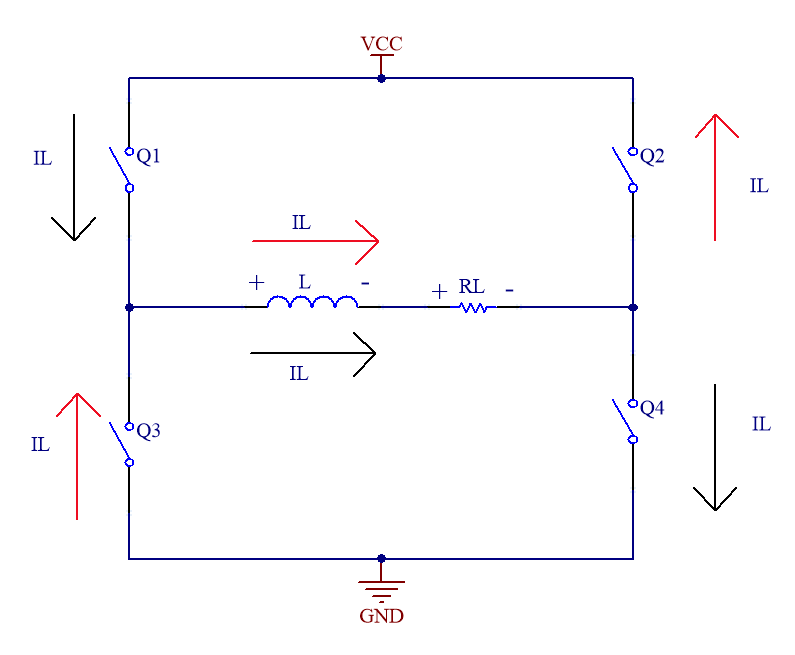
\includegraphics[scale=0.5]{puente_con_llaves.png}
	\caption{Topología simplificada.}
	\label{fig:img_topologia_simplificada}
\end{figure} 



El electroimán se conecta entre los puntos medios de cada par de llaves. De esta manera, la corriente puede circular en ambos sentidos, según se desee. Para esta aplicación en particular, la fuerza magnética es siempre en el mismo sentido, independientemente del sentido en que circule la corriente del electroimán. Por lo tanto, se adopta como sentido de circulación positivo de izquierda a derecha.

Para que la corriente circule en el sentido adoptado, se deben cerrar a la vez las llaves $Q_1$ y $Q_4$. La corriente comenzará a crecer como se muestra en la figura \ref{fig:img_corriente_exponencial}. Luego, para generar el periodo de decrecimiento, se abren estas llaves y se cierran $Q_2$ y $Q_3$. La corriente seguirá circulando en el mismo sentido, pero la alimentación del electroimán alternó su polaridad, por lo tanto la corriente tendrá una pendiente negativa. \colorbox{red}{se puede exxplicar mejor}
Es importante tener en cuenta que sólo se permite que dos llaves se enciendan a la vez, y esto se realiza de manera diagonal. Es decir, en la figura \ref{fig:img_topologia-puenteH}, $Q_1$ y $Q_4$ pueden estar encendidos, mientras que $Q_3$ y $Q_2$ están apagados, y viceversa. De otra forma, se podría generar un cortocircuito entre la fuente de alimentación y GND, que produciría una circulación de corriente denominada \textsl{shoot-through}. Esto debe ser tenido en cuenta al momento de diseñar el circuito.

Como se menciono previamente, para poder generar una corriente triangular con un valor medio deseado es necesario controlar el tiempo que se le aplica cierta polaridad de tensión al electroimán. Para poder controlar dicha polaridad, se debe actuar sobre las llaves en función de si se desea aumentar o disminuir el valor medio de la corriente. 

Una manera de hacerlo es mediante un circuito que compare la corriente de referencia q con la corriente que está circulando por el electroimán. De esta forma, si la corriente es menor a la de referencia, la polaridad de la tensión aplicada en los bornes del electroimán, será positiva. En cambio, si resulta mayor, será negativa. De esta forma, la corriente aumenta y disminuye respectivamente. Por lo tanto se plantea el siguiente diagrama\ref{fig:img_diag-en-bloques-comparador-sin-hist}:

\begin{figure}[H]
	\centering
	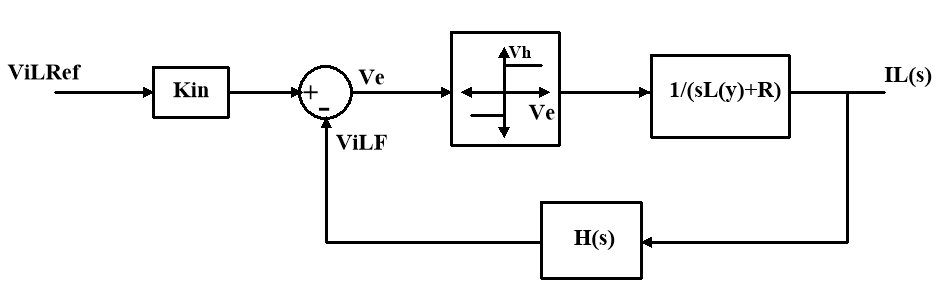
\includegraphics[width=\textwidth]{Diagrama-en-bloques-comparador-sin-hist.png}
	\caption{Diagrama en bloques simplificado del controlador de corriente.}
	\label{fig:img_diag-en-bloques-comparador-sin-hist}
\end{figure}

Con el circuito planteado hasta ahora, una vez que la corriente del electroimán(IL(s)) supere infinitesimalmente a la referencia, se produciría una conmutación en la polaridad de tensión aplicada al electroimán. Lo mismo sucedería cuando sea infinitesimalmetne menor. Esto produciría conmutaciones extremadamente rápidas en torno al valor medio y sería necesario alta velocidad en conmutación. Por lo tanto, para evitar esas oscilaciones, es necesario agregar un retraso de tiempo para evitar que la fuente conmute de forma indeseada.

Una manera de hacerlo es mediante un comparador con histéresis. Este bloque compara la corriente de referencia con la que está circulando por el electroimán y permite definir un ancho de histeresis. De esta forma en caso de que esta última sea menor que la referencia, la polaridad de tensión aplicada al electroimán será positiva y, por ende, la corriente aumentara hasta alcanzar la referencia. Una vez superada la referencia, se volverá a cambiar la polaridad en el electoimán, pero esta vez será negativa, haciendo que el valor medio de la corriente disminuya. Debido a que lo unico que cambia es el valor de tension en modulo con el que se exita al electroiman la constante de tiempo del circuito no cambia. Esto da como resultado a que la corriente oscile sobre un valor medio de forma triangular. El valor de el ripple de corriente esta determinado por el periodo de conmutacion de la fuentes. Estos parametros pueden ser definidos ajustando el ancho de histeresis. 

Finalmente se obtiene un modelo en bloques del sistema como se ve en la figura \ref{fig:img_diag-en-bloques}.

\begin{figure}[H]
	\centering
	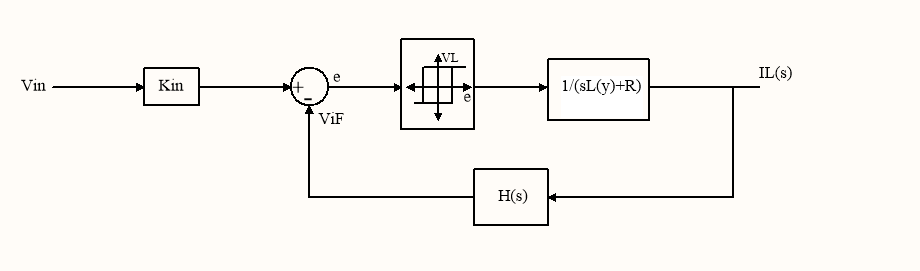
\includegraphics[width=\textwidth]{Diagrama-en-bloques.png}
	\caption{Diagrama en bloques simplificado del controlador de corriente.}
	\label{fig:img_diag-en-bloques}
\end{figure}


